\section{Experiments}
\label{sec:simResults}

We simulate the system shown in Fig. \ref{fig:juicyj}, where the car is modeled by the dynamics of Eq. \eqref{eq:cardynamics}, the controller is given by Eq. \eqref{eq:controller}, and the supervisor optimizes Eq. \ref{eq:cost_runtime} as explained in Section \ref{sec:evaluation}. 
The controller experiences a delay when receiving update values of $x_m$ and $x_v$. 
This is the computation delay computed offline during the profiling stage. 
The simulation is repeated three times: once for each choice of $\alpha$ from Eqs. \eqref{eq:f1}, \eqref{eq:f2} and \eqref{eq:f3}.
We also simulate two more scenarios: one where the schedule and frequencies are fixed at the highest throughput (highest power) values, and one where they are fixed at the lowest throughput (lowest power) values.

We initialize the robot aligned to the corridor $\theta=0$ but off from the center by 0.25m, i.e. $x=0.25$. 
The controller attempts to bring the robot to the middle of the corridor and align it with the corridor while the supervisor decides the hardware operating mode ($\sigma,F_c,F_g$) as per Sec. \ref{sec:scheduling}. 
At 10 seconds, we apply a steering disturbance to the system, which is a pulse of magnitude 3 degrees per second and a duration of 2 seconds. 
The controller again tries to recover from this disturbance while the supervisor picks the best operating mode for the perception algorithm. 

Figs. \ref{fig:cpuf} and \ref{fig:gpuf} show the selected CPU and GPU frequency versus time respectively. 
Fig. \ref{fig:power} show the computation power vs time, while Fig. \ref{fig:schedule} shows the schedule $\sigma$ of CPU-GPU allocation for tasks.
Fig. \ref{fig:xvst} shows the trajectory of $x$ versus time.  
Note that only the trajectory of $x$ for the lowest power, or highest delay mode differs enough from the others so as to be different visually in this plot.


\begin{figure}[t]
\centering
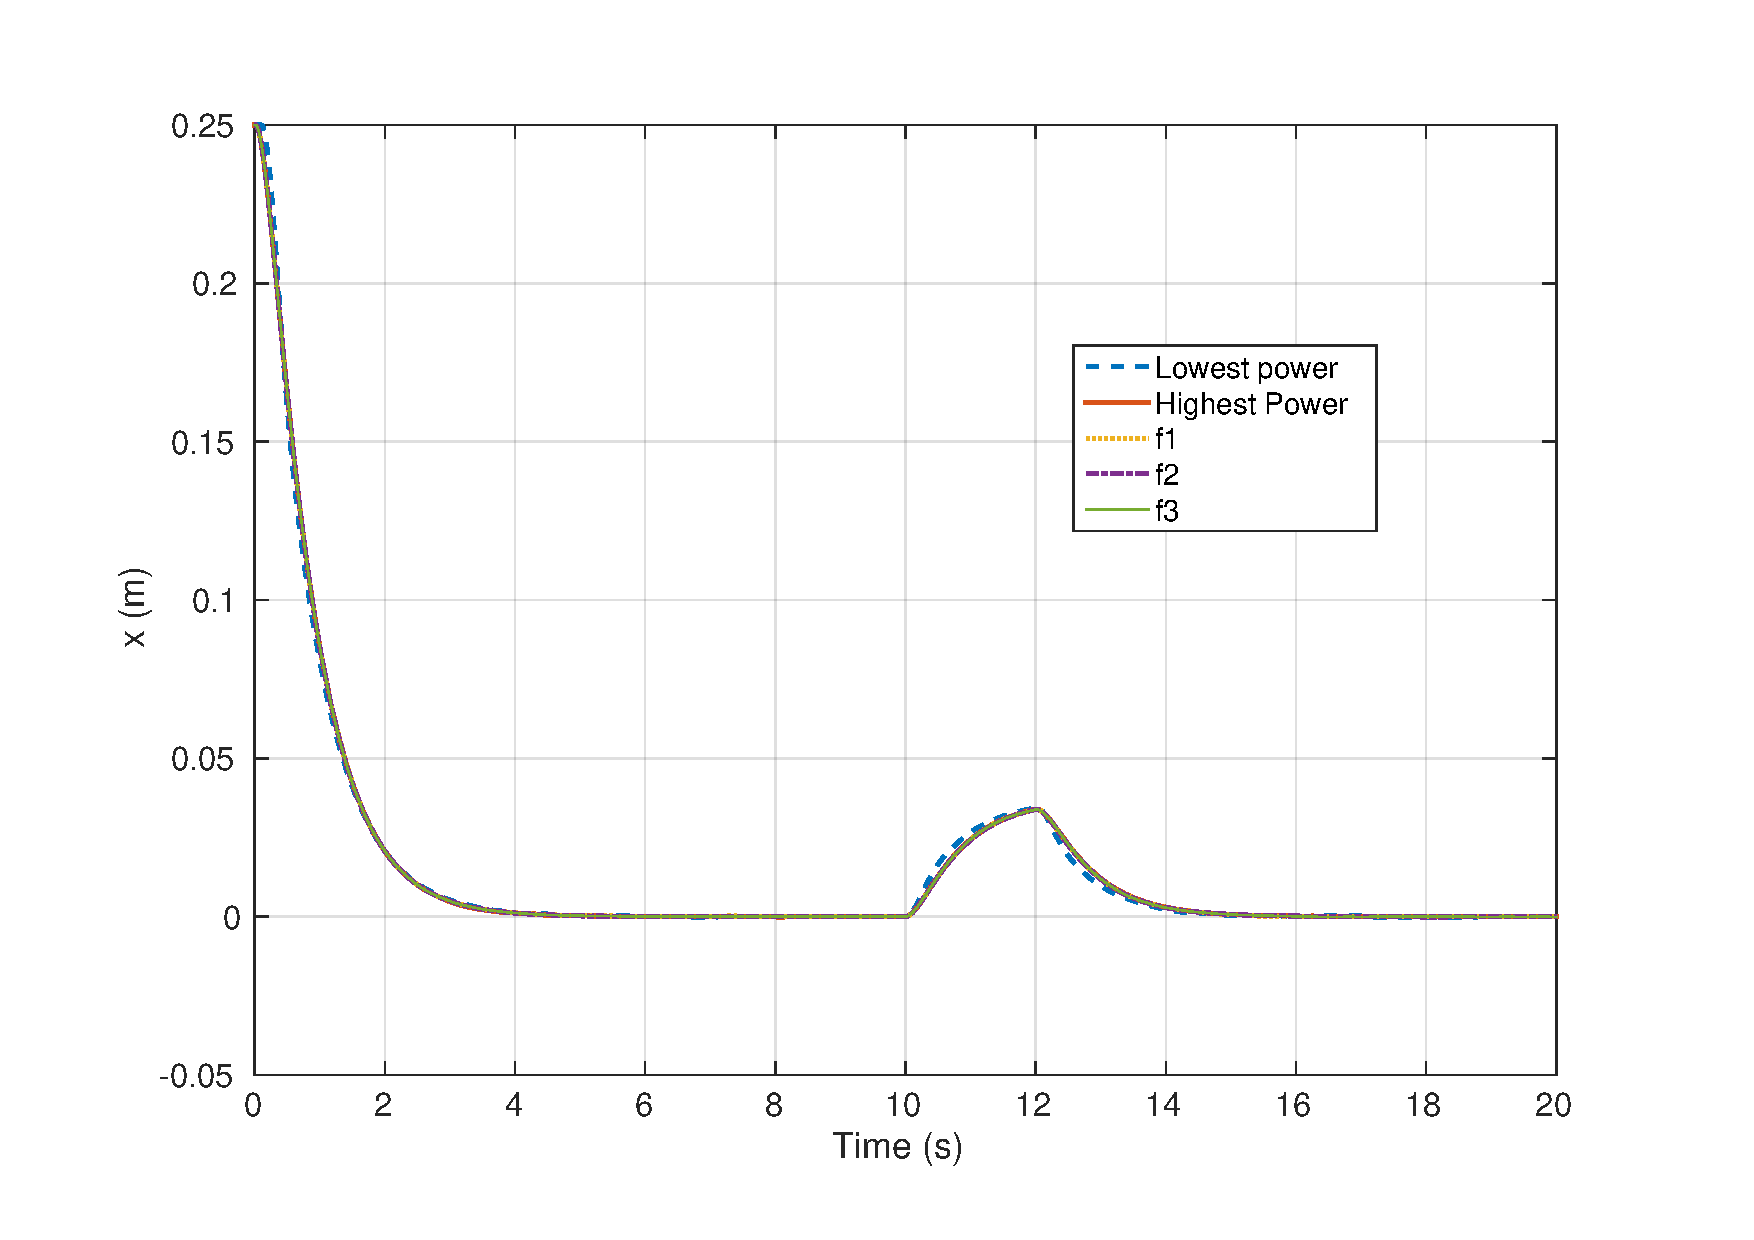
\includegraphics[width=0.49\textwidth]{../simulations/figs/xvst.pdf}
\vspace{-20pt}
\caption{$x$ position of the robot. Note, for modes other than the lowest power (most delay), the trajectory of x is very similar. This is also shown in table \ref{tbl:performance}}.
\label{fig:xvst} 
\end{figure}

To better understand these figures, let us go through 5 checkpoints (\textbf{a}, \textbf{b},\textbf{c}, \textbf{d} and \textbf{e}) in time common to Figs. \ref{fig:xvst}, \ref{fig:cpuf}, \ref{fig:gpuf}, \ref{fig:schedule} ,\ref{fig:power}.
At checkpoint \textbf{a} the controller starts to stabilize $x$ initial displacement of 0.25m. 
At this time, both $x_v$ and $x_m$ have high magnitudes, implying $\alpha$ takes a high value (close to 1) for all $f_i,\text{ }i=1,2,3$. 
Due to this, Fig. \ref{fig:schedule} shows that $\sigma$ becomes $CCG$ and Figs. \ref{fig:cpuf} and \ref{fig:gpuf} show that CPU and GPU frequencies are high, this implies the vanishing point algorithm is near its highest throughput. Correspondingly, Fig. \ref{fig:power} shows that the computation power is also high.

At checkpoint \textbf{b} $x$ has a small magnitude and is near settling the middle of the corridor. Because of this, both $x_v$ and $x_m$ have smaller magnitudes, and so $\alpha$ is small and the requested CPU and GPU frequencies start to decrease. $\sigma$ is still $CCG$ for all supervisory functions except $f_2$, but settles to $CCC$ for all 3 as $x$ settles to zero shortly after checkpoint \textbf{b}.

Checkpoints \textbf{c}, \textbf{d}, and \textbf{e} show how the system responds to a pulse-like disturbance in the steering (lasting from 10s to 12s). It is interesting to see how the different supervisory functions $f_i$ result in different switching between schedules CCC and CCG and different CPU and GPU frequencies.

 
\begin{figure}[t]
\centering
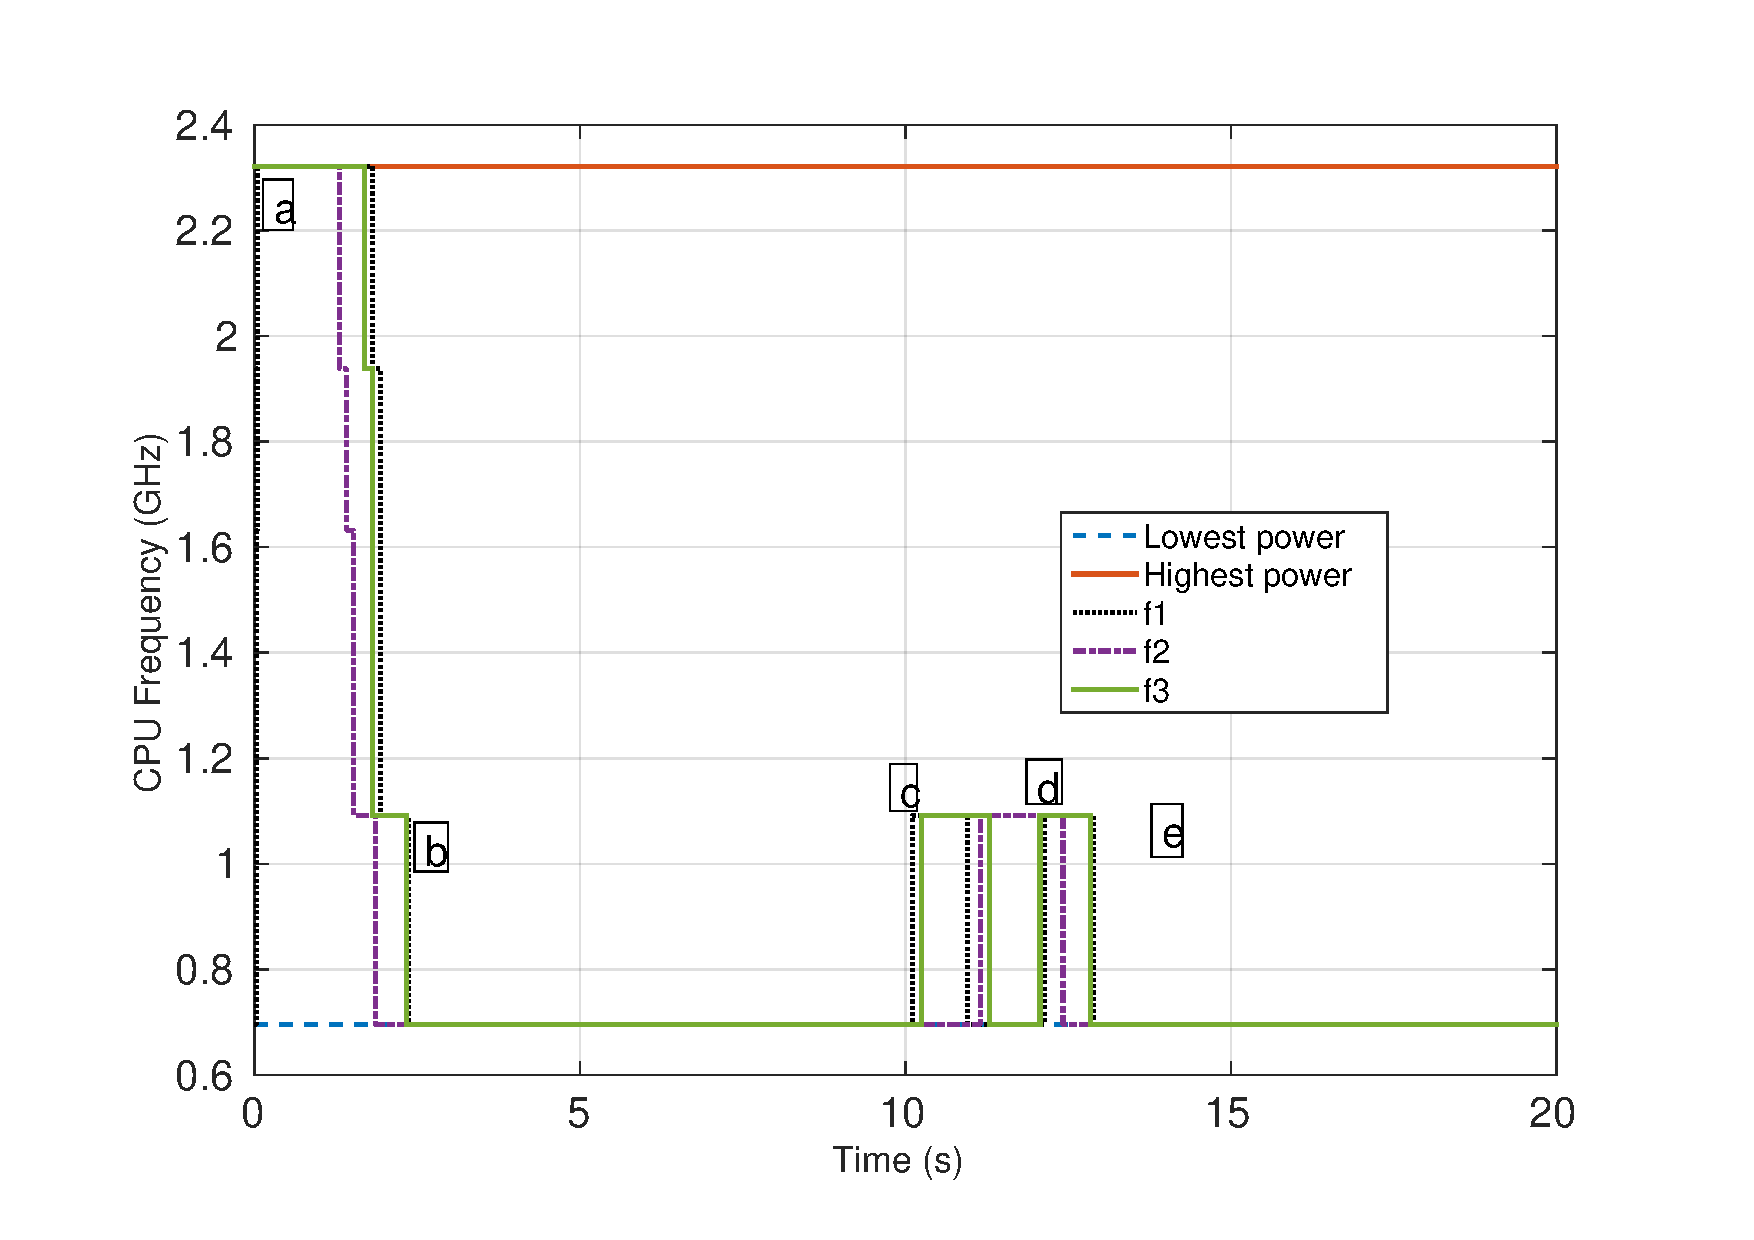
\includegraphics[width=0.49\textwidth]{../simulations/figs/CPUF.pdf}
\vspace{-20pt}
\caption{CPU Frequency selected versus time.}
\label{fig:cpuf} 
\end{figure}


\begin{figure}[t]
\centering
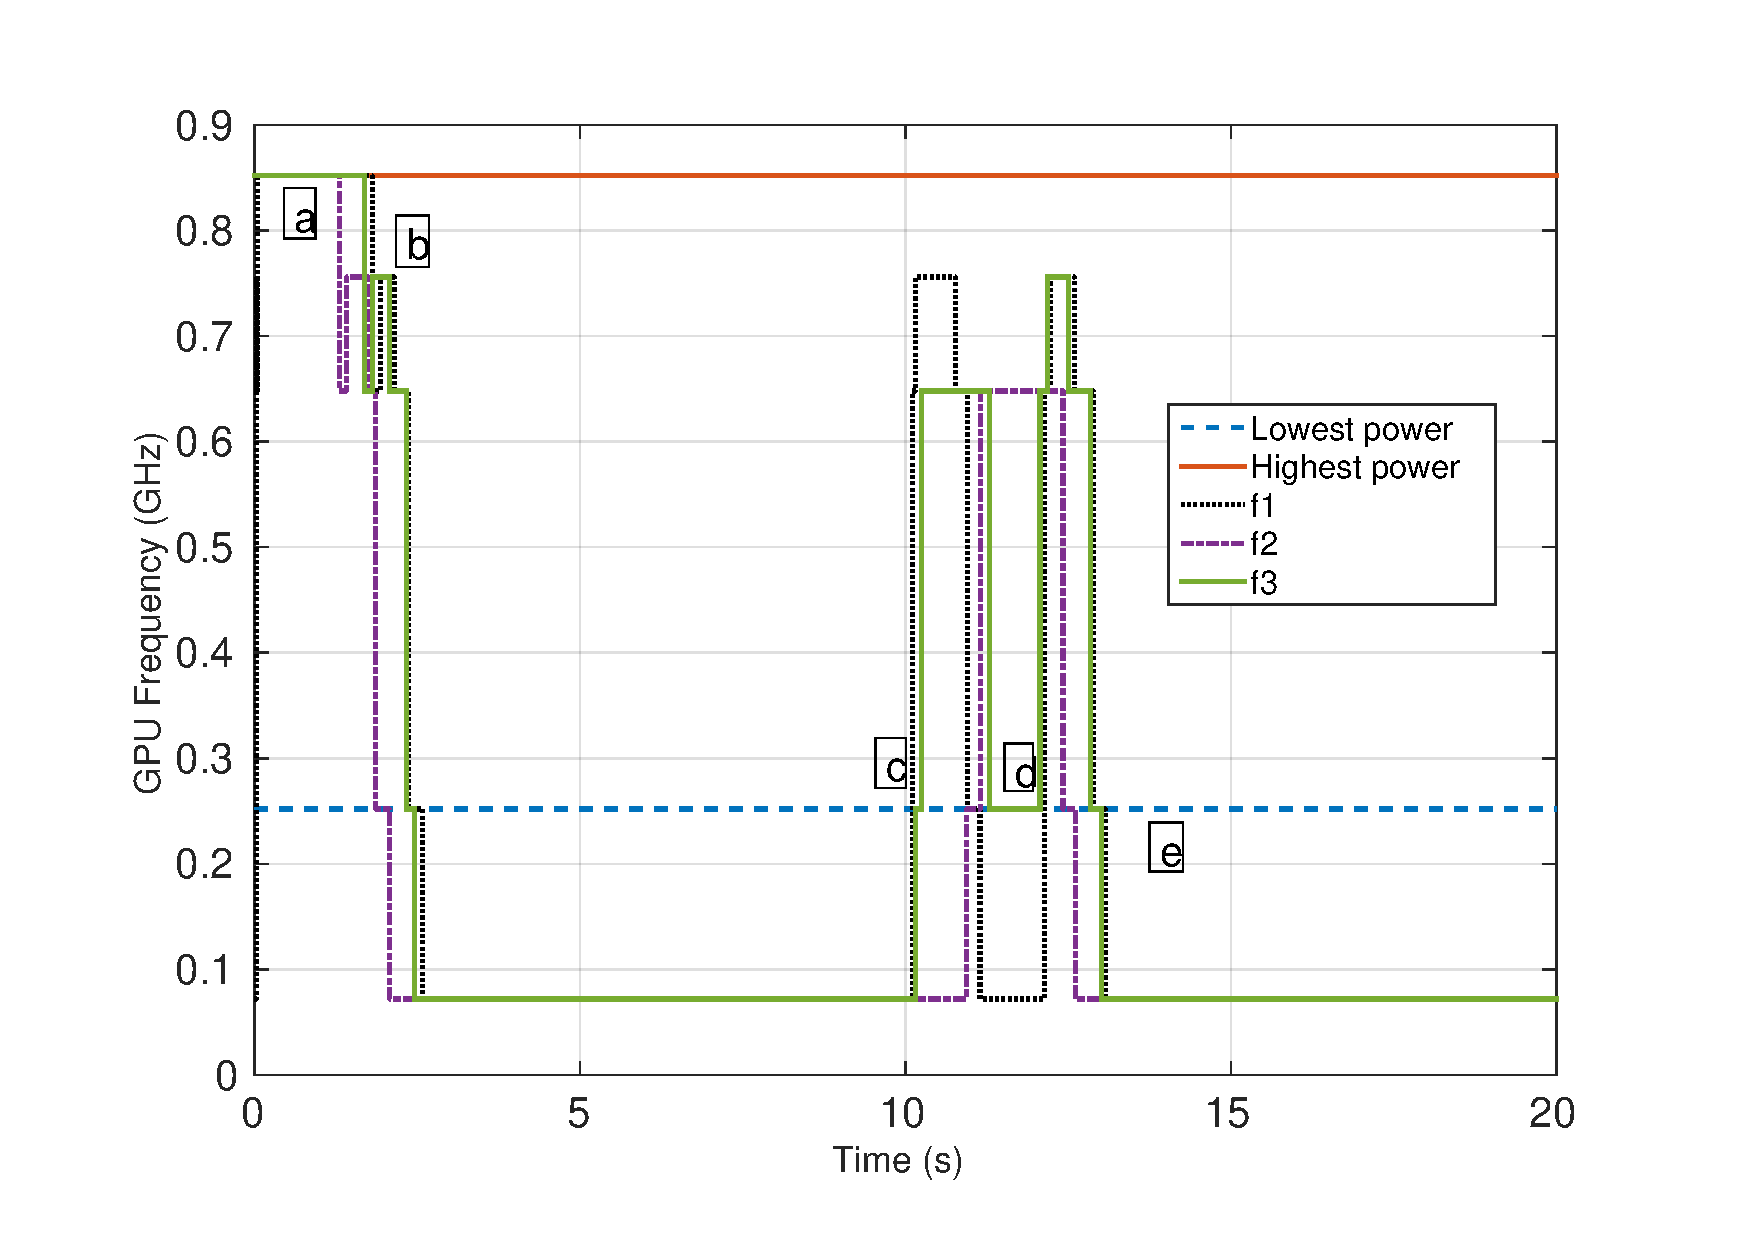
\includegraphics[width=0.49\textwidth]{../simulations/figs/GPUF.pdf}
\vspace{-20pt}
\caption{GPU Frequency selected versus time. Note, for the lowest power mode, the GPU is at its second lowest frequency and not the lowest (while the schedule is $\sigma=CCC$). This is because of the noise in power data while the GPU frequency is being changed while it is not computing any tasks.}
\label{fig:gpuf} 
\end{figure}


\begin{figure}[t]
\centering
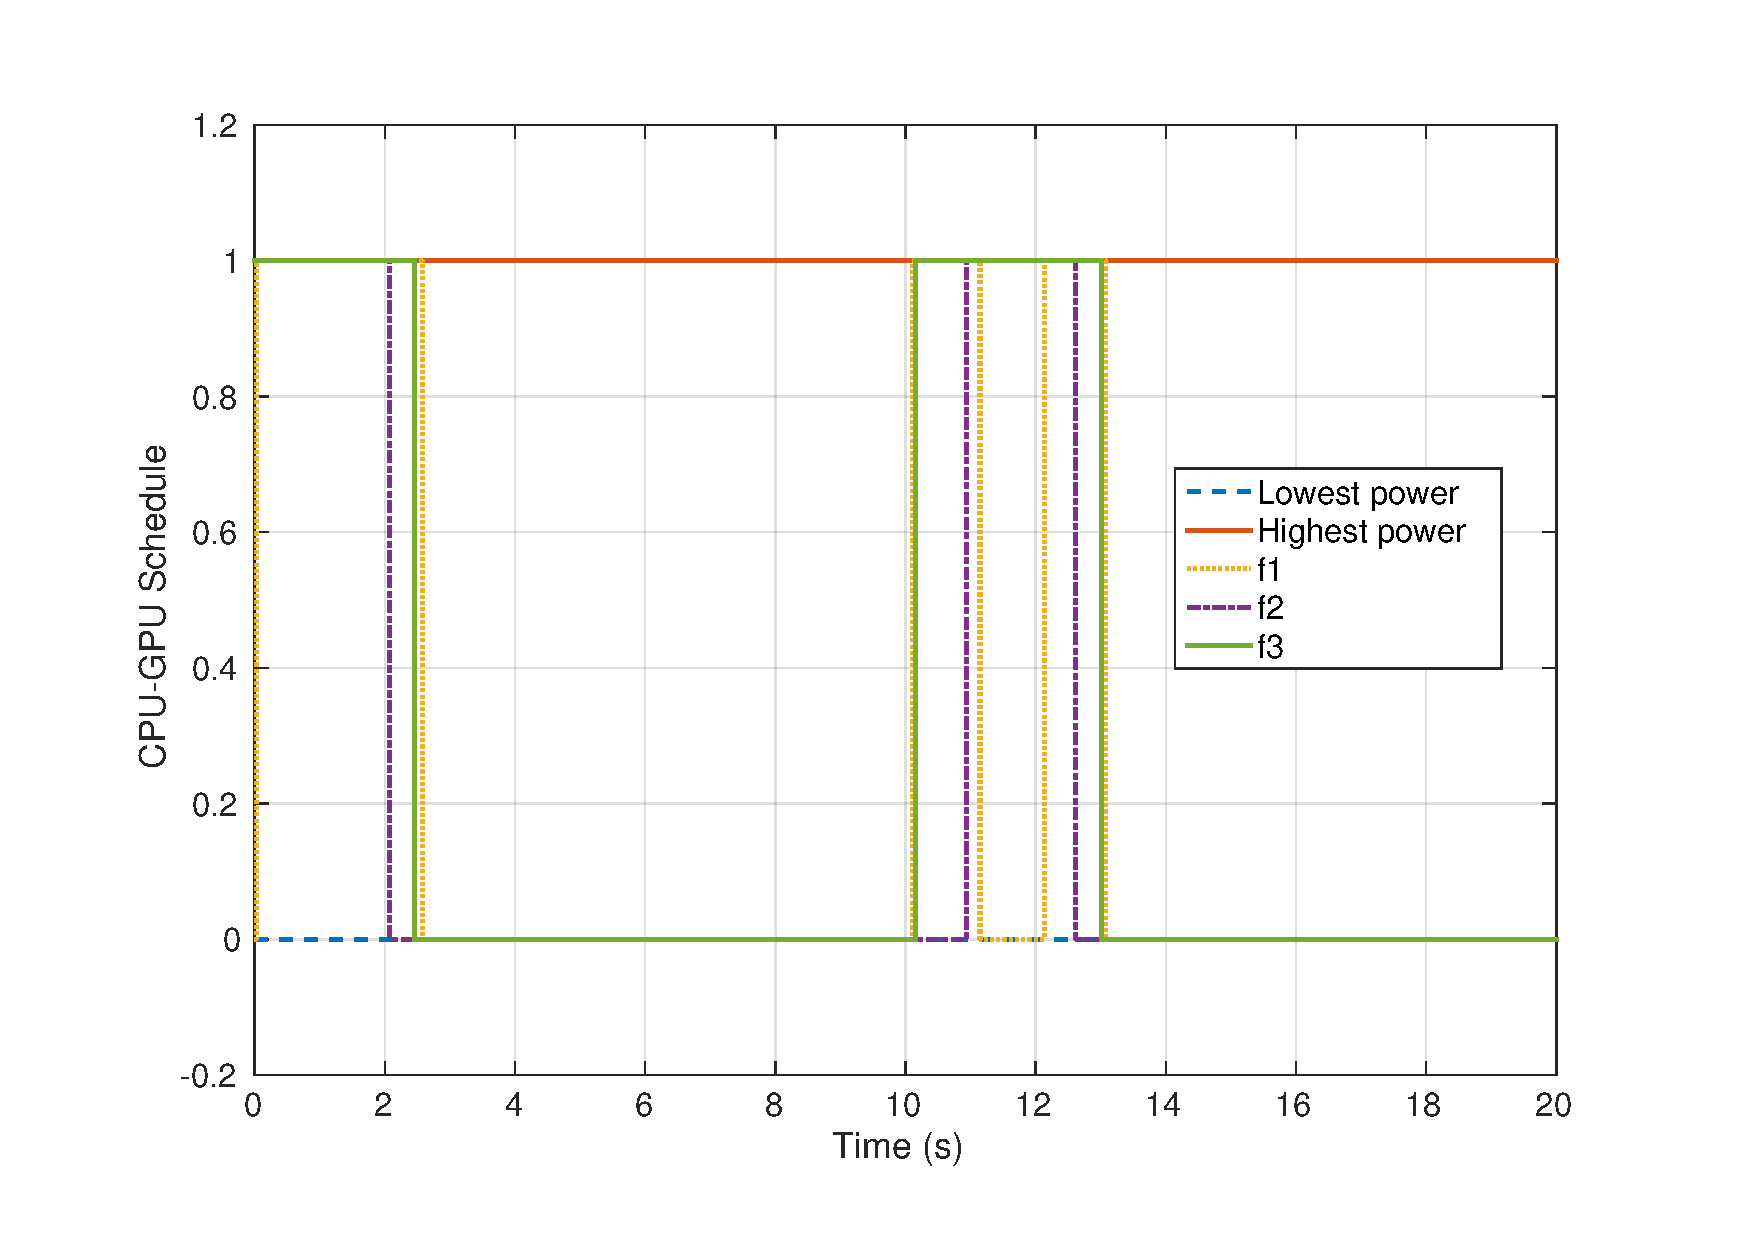
\includegraphics[width=0.49\textwidth]{../simulations/figs/schedule.pdf}
\vspace{-20pt}
\caption{Resource allocation schedule for the vanishing point algorithm. Note, the schedule switches between only two allocations. This is because the allocation $\alpha=CCG$ has the best throughput while having a relatively low power consumption, while $\alpha=CCC$ has the lowest power consumption. See the results in section \ref{sec:profiling} to get a better idea.}
\label{fig:schedule} 
\end{figure}

\begin{figure}[t]
\centering
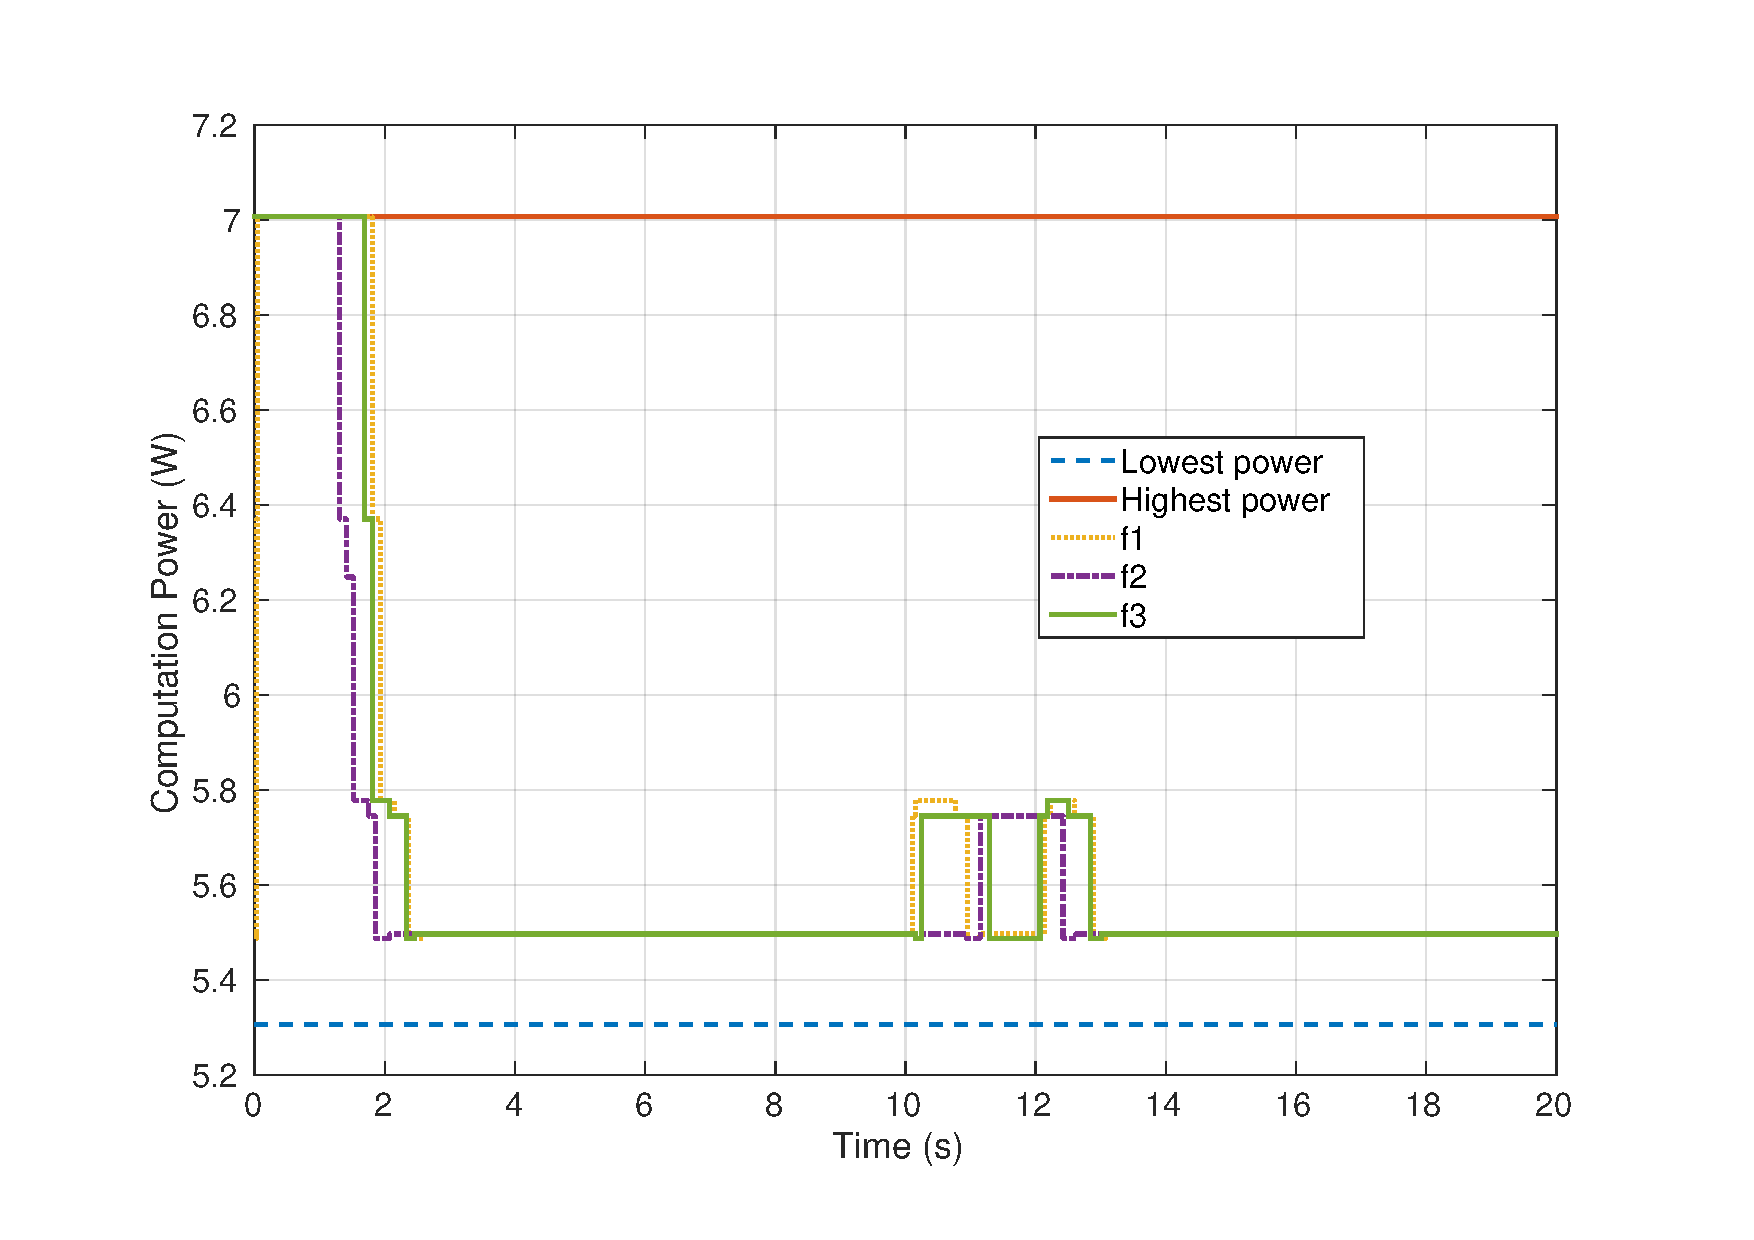
\includegraphics[width=0.49\textwidth]{../simulations/figs/power.pdf}
\vspace{-20pt}
\caption{Average computation power for running VP.}
\label{fig:power} 
\end{figure}

The closed loop control performance can be measured over a simulation time of $T$ seconds as $L = \int_0^T |x(t)|dt$, 
and the expected energy consumed is calculated as the sum of powers over $T$ seconds.
A summary of the control performance and computation energy consumed for these five cases is shown in table \ref{tbl:performance}. It is clear that operating with the highest power/lowest delay mode for the vanishing point results in the best control performance, but the computation energy is high. On the other hand, lowest power/highest delay mode results predictably in low power consumption and the worst control performance. With out two stage approach, control performance is very similar (less than $1\%$ degradation) to the highest power mode, while the computation energy is significantly (about $20\%$) lower. This clearly shows the benefit of our approach.

\begin{table}[htb]
\begin{center}
\caption{Control performance and computation energy}
\label{tbl:performance}
\begin{tabular} {|c|c|c|}
	\hline
	\textbf{Supervisor} & \textbf{Control perf.}(L) & \textbf{Energy}(J) \\ \hline
	Lowest power (mode fixed) & 0.3245 & 106.12  \\ \hline
	Highest power (mode fixed) & 0.3010 & 140.13  \\ \hline
	 $f_1(x_v)$ & 0.3025 & 113.16  \\ \hline
	 $f_2(x_m)$ & 0.3023 & 112.39 \\ \hline
	 $f_3(x_v,x_m)$ & 0.3018 & 113.07 \\ \hline
	 
\end{tabular}
	\vspace{-10pt}	
	\end{center}
\end{table}


